\section{Requirements}
\labelsec{Requirements}
A differential drive robot (called from now on robot) must reach an area (B) starting from a given point A. To reach the area B, the robot must cross an area equipped with N (N>=1) distance sensors (sonars). The signal emitted by each sonar is reflected by a wall put in front of it at a distance of approximately 90 cm.
Design and build a (prototype of a) software system such that:
\begin{itemize}
	\item shows the sonar data on the GUI associated to a console running on a conventional PC
	\item evaluates the expression: \\
			$ (s_{k} + s_{k+1} + ... s_{N}) / (N-k+1) $ \\
			where k is the number of the first sensor not reached by the robot and sk is the value of the distance currently measured by that sensor. If the value of the expression is less than a prefixed value DMIN( e.g. DMIN=70), play an alarm sound.
	\item when the robot reaches the area in front of a sonar, it
			\begin{enumerate}
				\item first stops
				\item then rotates to its left of approximately 90 degrees
				\item starts blinking a led put on the robot
				\item takes a photo of the wall (in a simulated way only, if no WebCam is available) and sends the photo to console by using the MQTT protocol
				\item rotates to its right of approximately 90 degrees to compensate the previous rotation
				\item stops the blinking of the led and continues its movement towards the area B
			\end{enumerate}
	\item when the robot leaves the area in front to the last sonar, it continues until it arrives at the area B
	\item stops the robot movement as soon as possible:
	\begin{itemize}
		\item when an obstacle is detected by the sonar in front of the robot
		\item when an alarm sound is played
		\item the user sends to the robot a proper command (e.g. STOP)
	\end{itemize}
	\item makes it possible to restart the system (by manually repositioning the robot at point A) without restarting the software
\end{itemize}

\begin{figure}[h]
	\centering
	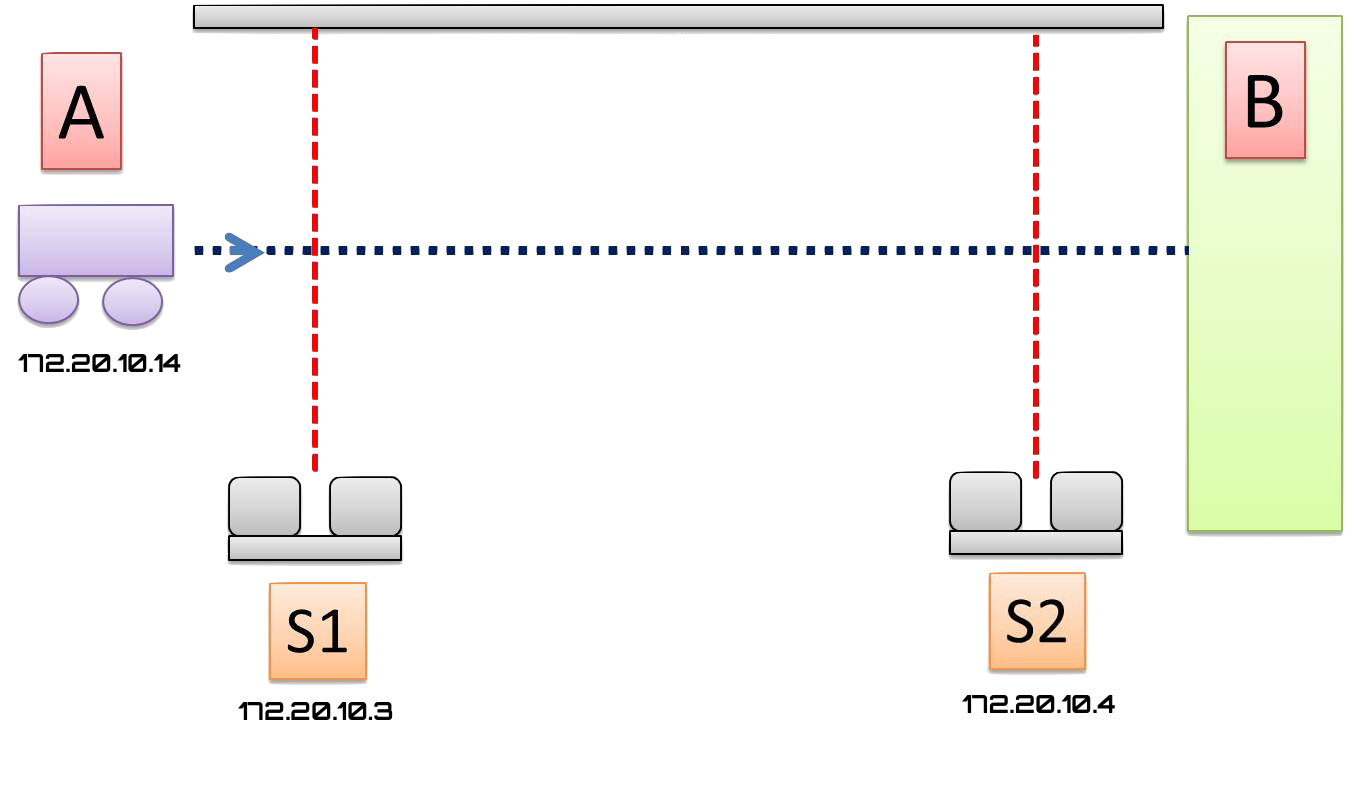
\includegraphics[width=\linewidth]{system.png}
\end{figure}
